\section{Moving stars: waiting is a resource}
\label{sec:moving}

\paragraph{A temporal graph with closed-form edges.} Under linear motion the
separation of stars $i$ and $j$ is
$d_{ij}(t)=\lvert p_{ij}+w_{ij}t\rvert$, where $p_{ij}$ is the relative position
at $t=0$ and $w_{ij}$ the relative velocity. Since $d_{ij}^2$ is a convex
quadratic in $t$, a hop of range $r$ is open on \emph{exactly one} interval
$[a_{ij},b_{ij}]$, found in closed form. A ship cruising at $v$ intercepts a
moving target after $\tau$ solving $\lvert p+w\tau\rvert=v\tau$. We open the
edge when $d_{ij}(t)\le r(1-\lvert w\rvert/v)$, which guarantees a flown
distance $\le r$. A colony at $i$, ready at time $t$, leaves at
$\max(t+s,a_{ij})$ if that is $\le b_{ij}$, where $s$ is an optional settling
delay. Leaving later never arrives earlier, so the network is FIFO and
Dijkstra over arrival times is exact \cite{kaufman1993fastest}. Candidate pairs
come from time-sliced KD-tree queries. A unit test checks that no pair whose
separation ever drops below $r$ is missed. A second test checks the arrival
times against a Bellman--Ford fixed point. One run per $r$ yields reach at
every horizon $T$ at once. With $r\le2.25$~pc and $T=1$~Myr the graph has
\TdPairs\ candidate pairs.

\begin{figure*}[t]
\centering
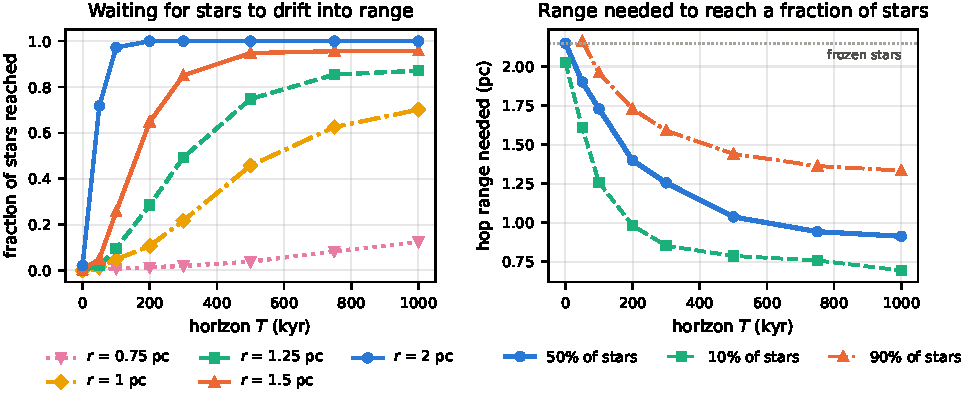
\includegraphics[width=\textwidth]{figures/moving.pdf}
\caption{Moving stars, \TdNEval\ stars within \TdEval~pc, ships at \TdVship~$c$.
\textbf{Left:} fraction reached by horizon $T$ for several hop ranges. Below
the frozen threshold, reach grows steadily as stars drift into range.
\textbf{Right:} range needed to reach 10/50/90\% of stars by time $T$. The band
is the spread over \TdNBoot\ astrometric bootstrap draws. The frozen-star value
is the dotted line.}
\label{fig:moving}
\end{figure*}

\paragraph{Waiting lowers the threshold substantially.} Figure~\ref{fig:moving}
is the central result. If a colony may wait up to 100~kyr, the range needed to
reach half the stars falls from \RFifty\ to \RFiftyTHundred~pc, a
\RedHundred\% reduction (bootstrap range \RedLoHundred--\RedHiHundred\%). The
reduction is \RedTwoHundred\% within 200~kyr, \RedFiveHundred\% within 500~kyr
($r_{50}=\RFiftyTFiveHundred$~pc) and \RedThousand\% within 1~Myr. Our
falsification criterion, a reduction below 5\% at every horizon up to 10~Myr,
is decisively rejected. Stellar motion is not a correction to interstellar
routing. Over $10^5$-year horizons it dominates.

\paragraph{The stars carry the front.} For sub-threshold ranges the expansion
speed is set by stellar motion, not by the ship. With $r=1$~pc, half the stars
within \TdEval~pc are reached at an effective speed of \FrontOne~pc/Myr
(\FrontOneKms~km/s), comparable to the local velocity dispersion. With
$r=1.5$~pc it is \FrontOneHalf~pc/Myr. Naively extrapolated across a
30-kpc Galaxy, these give \GalaxyCrossGyrOne\ and \GalaxyCrossGyrOneHalf~Gyr,
far shorter than the Galaxy's age. This is the Carroll-Nellenback et al.\
\cite{carroll2019fermi} conclusion, obtained here from explicit routes on
measured stars.

\paragraph{What slows it down.} \emph{Settling time} matters most. At
$r=\SweepR$~pc and $T=200$~kyr, \SettleZero\% of stars are reached with
instant relaunch, \SettleTen\% if each colony needs 10~kyr before it can
launch again, and \SettleHundred\% with 100~kyr. \emph{Ship speed} matters less
than one might think: \SpeedMid\% at 0.01~$c$ versus \SpeedFast\% at 0.1~$c$.
Only at 0.001~$c$ (300~km/s, comparable to stellar motions) does reach
collapse, to \SpeedSlow\%.

\paragraph{Boundary check.} Stars that would enter from beyond the catalogue
are missing, so a catalogue-limited run \emph{underestimates} the benefit of
motion. The count of catalogued stars inside \TdEval~pc stays at
\RetFiveHundred\% of its initial value at 500~kyr and drops to \RetThousand\% at
1~Myr. Results beyond 500~kyr are therefore conservative. The full
configuration uses the 100-pc catalogue.
